\cotefile{83}
\scanpage{46}
\mspage{8}
Autre façon de le dire :

$\rho_{ijkl}$ ne dépend que du
``carré'' $(i,j)(k,l)$ muni d'une section
du produit contracté des \deleted{\illegible{1}}diagonales,
i.e. d'une codiagonale, car
\[
\deleted{\unsure{\mathrm{car}}}\quad
\rho_{(i,j)(k,l)}=\rho_{(k,l)(i,j)}
\tag*{(9)}
\]
\figure{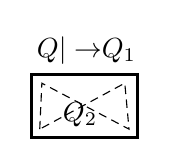
\begin{tikzpicture}[x=1.35cm,y=0.8cm]
\draw[very thick] (0,0) rectangle (1,1);
\draw[densely dashed] (0.08,0.13)--(0.10,0.86)--(0.92,0.13)--(0.88,0.86)--cycle;
\node[above] at (.52,1) {$\deleted{\unsure{Q|\rightarrow}}Q_1$};
\node at (.46,.36) {$Q_2$};
\end{tikzpicture}}
\margin{$Q_3$ est le troisième carré}

(\uline{NB} Cette relation n'a de sens que parce que
$\operatorname{End}(W)$ est supposé commutatif)

On se donne une \deleted{\unsure{carré|coin}} str. carr. ou
codiag. de $I$, $\sim$ se donner
un repère de l'ens $\operatorname{Car}(I)$ des
structures \unsure{carrées|carrés|coin}, et la donnée de
% slanted
\margin{\uline{vérifier la} \uuline{compatibilité}. Il faut peut-\unsure{ê} twister par un (\unsure{aut}) de $\mathfrak S_3$\ldots}
équivaut à une application de
\[
\underbrace{\operatorname{Rep}\operatorname{Car}(I)}_
{\substack{\text{torseur}\\\text{sous }\text{\uuline{$\mathfrak S_3$}}}}
\longrightarrow \unsure{\mathcal U|U}(k)
\]

Il reste à décrire la catégorie des
\unsure{quadrités|quadralités} dans $C$, \deleted{\unsure{la don}} de façon
plus simple que par un système
de $24$ flèches $u_{(i,j)(k,l)}$ deux à deux opposées.
% archive sheet number: 45
